 \chapter{\label{ch5-calibration}Calibration} 

\minitoc

\notes[inline,caption={}]{
	\section{Plan}
	\subsection{Topics}
	\begin{itemize}
		\item Pedestal subtraction
		\item Transfer functions
		\item Gain Matching
		\item SPE
		\item Flat fielding
		\item Time correction
		\item Future
		\begin{itemize}
			\item Live calibration
		\end{itemize}
	\end{itemize}
	\subsection{Questions}
	\begin{itemize}
		\item TARGET architecture diagram, Wilkinson ADC 
		\item How much detail about all the TF approaches do I go into?
	\end{itemize}
}


\change[inline]{Flow diagrams? See Cyril talk 18/07/06 camera calibration call}

\lstset{language=Python}

\section{Introduction}

In order to obtain meaningful and reliable results from the camera, a number of calibrations must be applied to the waveforms read. A primary objective of my DPhil is to investigate the most optimal and efficient approaches for these calibrations (in accordance with the \gls{cta} requirements described in Chapter~\ref{ch3-architecture}), and to determine if additional calibrations are required.

The calibrations applied have evolved during the course of the prototyping of \gls{chec}; the calibrations applied to \gls{chec-m} waveforms are not the same for \gls{chec-s}. Additionally, the calibration applied for the on-sky pipeline can differ from the calibration used to obtain results such as the charge resolution.

When I joined the \gls{chec} development, the calibration discussion was still in its infancy. Some approaches had been tested in a laboratory environment \cite{Bechtol2012}, but there had been little discussion on how exactly the calibrations could be applied efficiently in an analysis pipeline, where one might not be able to use the same detailed calibration due to limited resources (such as memory and time). A major contribution of my DPhil was to prototype the calibrations procedures, develop an approach for a calibration pipeline, write the software to perform such a pipeline, and finally assess the performance of the pipeline. This was an iterative procedure, the development of which is still ongoing. However, a procedure now exists that allows us to obtain meaningful results from the waveform data, a capability that is of paramount importance in the commissioning of the camera.

In this chapter I will outline each of the calibration steps that are presently adopted for \gls{chec}. They are introduced in the general order that they are applied, and split into the categories of \gls{target} \gls{asic}, photosensor, and "other" calibrations.

\section{TARGET Calibration}

The calibrations described in this section relate to the \gls{target} module. As detailed in Chapter~\ref{ch2-mechanics}, the \gls{target} \gls{asic} is responsible for the sampling, digitisation and readout of the waveform data. As a result there are two calibrations that are solely related to the \gls{target} \gls{asic}: electronic pedestal subtraction and the linearity correction via the transfer function. 

The functional block diagram of the \gls{target} \gls{asic} in Figure~\ref{fig:target5diagram} outlines the electronics responsible for the need of these calibrations, and should be used as a reference in the following descriptions.

As the calibrations in this section are very low-level, and related to \gls{chec}'s specific \gls{fee}, they are handled by the TargetCalib library (Chapter~\ref{ch4-software}).

\subsection{Electronic Pedestal Subtraction}

\the\textwidth

\begin{figure}
\begin{minipage}[t]{.49\textwidth}
  \centering
  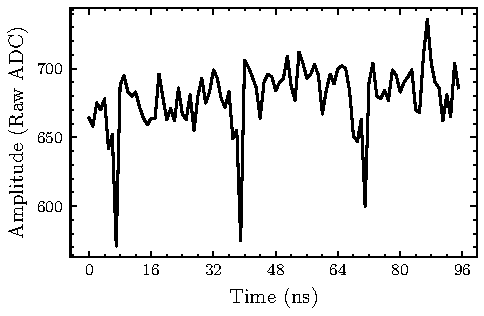
\includegraphics[width=0.92\textwidth]{rawwf_10} 
  \captionof{figure}[Raw waveform]{TARGET-C waveform as read out from CHEC-S, showing the electronic pedestal in the absence of any other input, before any calibration is applied.}
  \label{fig:rawwf}
\end{minipage}%
\hfill
\begin{minipage}[t]{.49\textwidth}
  \centering
  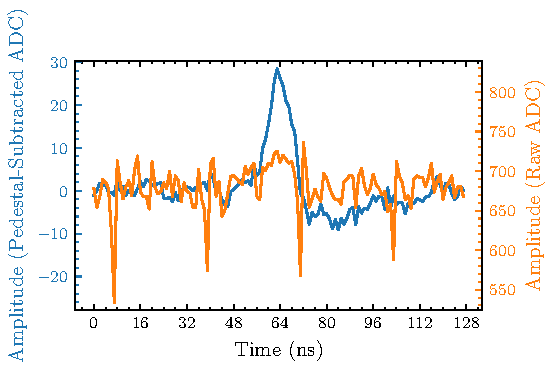
\includegraphics[width=\textwidth]{pulse_raw_vs_pedestal}
  \captionof{figure}[Comparison of pedestal-subtracted waveform with raw waveform]{CHEC-S waveform  containing a 5~p.e. pulse, before and after pedestal subtraction.}
  \label{fig:pulse_raw_vs_pedestal}
\end{minipage}
\end{figure}

\begin{figure}
  \begin{subfigure}[b]{0.49\textwidth}
    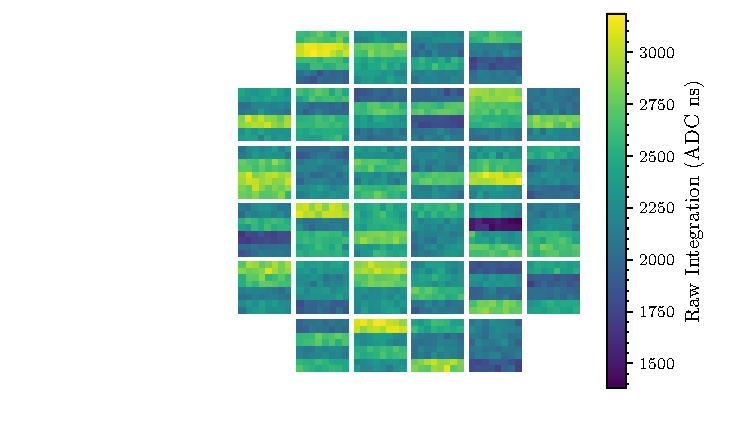
\includegraphics[width=\textwidth]{r0_cherenkov_image_mirrored_cropped}
    \caption{Raw image.}
    \label{fig:r0_cherenkov_image_mirrored_cropped}
  \end{subfigure}
  \hfill
  \begin{subfigure}[b]{0.49\textwidth}
    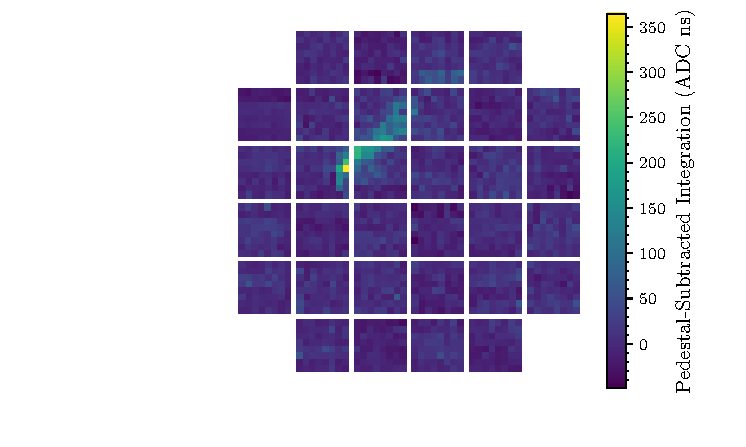
\includegraphics[width=\textwidth]{r1_cherenkov_image_mirrored_cropped}
    \caption{Pedestal-subtracted image.}
    \label{fig:r1_cherenkov_image_mirrored_cropped}
  \end{subfigure}
  \centering
  \begin{subfigure}[b]{0.49\textwidth}
    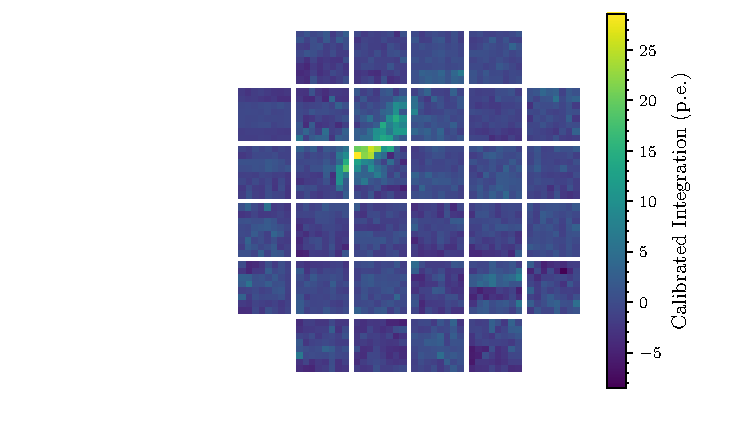
\includegraphics[width=\textwidth]{r1pe_cherenkov_image_mirrored_cropped}
    \caption{Final calibrated image.}
    \label{fig:r1pe_cherenkov_image_mirrored_cropped}
  \end{subfigure}
  \caption[Comparison of calibration stages with a Cherenkov shower image.]{The same image of a Cherenkov shower taken with CHEC-M, but at different stages of calibration. An integration window is chosen using the \textit{Neighbour Peak Finding} technique (Chapter~\ref{ch6-reduction}) on the p.e. calibrated waveforms. The same samples are then integrated for each of the calibration stages.}
\end{figure}

The most important, but also the simplest, calibration to apply is the subtraction of the electronic pedestal. Each cell in the storage array of the \gls{asic} is a unique capacitor. For a specific input \gls{vped}, each capacitor has its own resulting electronic pedestal value. As each sample of the waveform corresponds to a single storage cell, each sample therefore has a unique pedestal value to be subtracted. This is apparent in Figure~\ref{fig:rawwf} where the variation from sample-to-sample is very large. This variation is large enough that low-amplitude pulses (Figure~\ref{fig:pulse_raw_vs_pedestal}) and low-amplitude Cherenkov images (Figure~\ref{fig:r0_cherenkov_image_mirrored_cropped}) are undetectable in the camera. This variation in electronic pedestal is also apparent between pixels, and even more so between \glspl{asic}. As a result, the outlines of the \glspl{asic} are the dominating feature in camera images containing raw samples, such as Figure~\ref{fig:r0_cherenkov_image_mirrored_cropped}. With the pedestal subtraction alone, the waveforms are transformed into a state of which a moderate amount of Cherenkov shower assessment can be performed, as demonstrated in Figure~\ref{fig:r1_cherenkov_image_mirrored_cropped}.

\begin{figure}
	\centering
    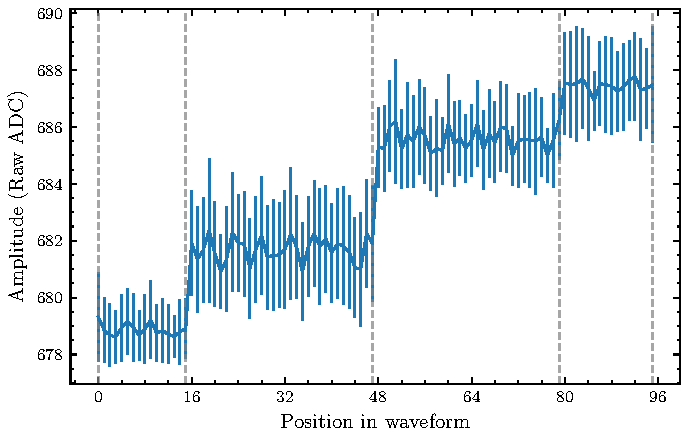
\includegraphics[width=\textwidth]{cellwf_15} 
	\caption[Storage-cell-amplitude dependence on position in the waveform.]{Average amplitude of the electronic pedestal for a single storage cell in a TARGET-C ASIC, at different positions in the waveform. Error bars indicate the standard deviation of the amplitudes. The grey dashed lines indicate the position of the block edges in the waveform for this cell. The average of the values inside each block segment equals the pedestal value stored in the lookup table for that cell, in each of those block positions.} 
	\label{fig:cellwf}
\end{figure}

There are $2^{14} = 16,384$ storage cells per channel (for \gls{chec-m}, $2^{12} = 4096$ for \gls{chec-s}\change{Make sure to mention about the difference in number of cells for checs in ch2}), therefore naively it could be concluded that there are $32 (Modules) * 64 (Channels) * 16,384 (Cells)$ pedestal values to keep record of. However, there is an additional contribution to the behaviour of the pedestal - discharging a cell to read out its value will slightly discharge adjacent cells. The result of this effect is that the further along in the waveform a cell is, the lower its pedestal value will be. This effect is reversed with \gls{targetc}, where the later blocks of the waveform are digitised first (Figure~\ref{fig:cellwf}). Consequently, an extra dimension of ``position in waveform'' needs to be considered.

\subsubsection{Generation}

In order to perform the pedestal subtraction, one must first generate a lookup table of pedestal values. This can be easily obtained with a calibration run where the voltages across the photosensor are disabled, and forcing the camera to trigger (with either an external pulse generator, or internally via software) to obtain a large amount of waveform data. Typically around 30,000 events provide enough samples for every storage cell, in every waveform position, to be hit at least 10 times. The samples are then collected as a running average with the dimensions $[Module, Channel, Starting Block, Blockphase+Sample\_i]$, where the $Starting Block$ is the storage block that the first sample in the waveform belongs to (see Figure~), $Blockphase$ is the cell index within the storage block that the waveform begins on, and $Sample\_i$ is the index of each sample in the waveform. This is illustrated in Figure~\change{include figure, and edit to use bp 8 and 12}, where for these two readout windows shown, the pedestal running average |Pedestal[TM][CHANNEL][9][8:103]| and |Pedestal[TM][CHANNEL][8][12:107]| will be contributed to, respectively.

The TargetCalib library handles the pedestal lookup table generation, and stores it into a \gls{fits} file. A new pedestal file is typically generated at the start of each new dataset, as the dependencies on temperature and evolution with time are still being investigated.

\subsubsection{Application}

To apply the pedestal, the entry within the lookup table that corresponds to each sample is subtracted from the waveform. The result of the subtraction can be seen in Figures~\ref{fig:pulse_raw_vs_pedestal}~\&~\ref{fig:r1_cherenkov_image_mirrored_cropped}. 

\subsubsection{Performance}

\begin{figure}
	\centering
    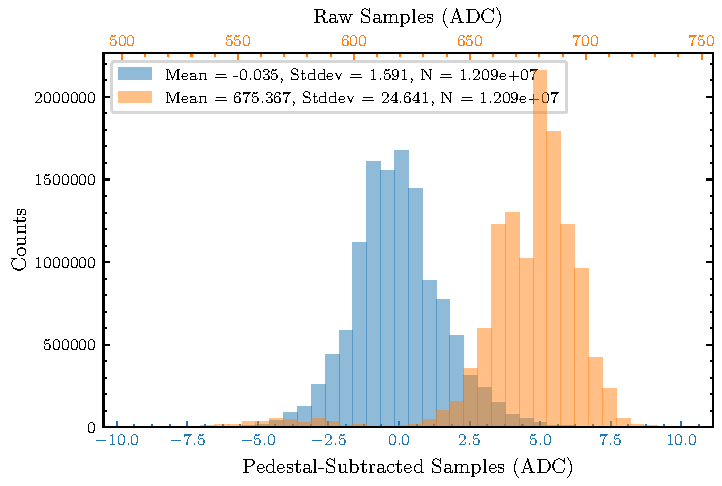
\includegraphics[width=\textwidth]{pedestal_hist} 
	\caption[Spread of electronic-pedestal values before and after the pedestal subtraction.]{Spread of electronic-pedestal values before and after the pedestal subtraction for a single TARGET-C channel. The waveforms used to create the pedestal lookup table are separate to those used in these histograms.} 
	\label{fig:pedestalresiduals}
\end{figure}

The primary quantification of this calibration's performance is the standard deviation of electronic-pedestal samples that have had separately-created pedestal values subtracted from them. Figure~\ref{fig:pedestalresiduals} demonstrates the performance of the pedestal subtraction for a \gls{targetc} channel, achieving a residual variation of 1.6~ADC (approximately 0.5~p.e.).

\subsection{Transfer Function}

The other calibration related to the digitisation and readout inside the \gls{target} \gls{asic} is caused by the non-linearities in the storing and reading of charge to and from the storage cells. The components responsible for the need for this calibration are the sampling array, gain/buffer amps, and the Wilkinson \glspl{adc}, seen in Figure~\ref{fig:target5diagram}. The non-linearity of these components is propagated to the sample readout - a sample with twice the amplitude input into \gls{target} will have less than twice the amplitude when readout.

To correct for this non-linearity, a look-up table is generated to convert from the sample amplitude read-out (in ADC), to the input sample amplitude (in mV). This look-up table is known as the Transfer Function. As one might expect, each sampling cell has its own linear response to correct for, and therefore a look-up table is typically required at-least per channel and per sampling cell, however a noticeably improved performance is observed by considering a Transfer Function per storage cell \change{need to show this, maybe in TF Investigations appendix?}.

There are two forms of Transfer Function that have been considered for \gls{chec}, distinguished by the type of input used to generate them. A \gls{dc} Transfer Function is created by applying a constant \gls{dc} input of known voltage into the module, and iterating over the full dynamic range by varying the voltage. An \gls{ac} Transfer Function is generated by inputting a pulse of a known amplitude with a shape expected from the photosensor, and iterating as with the \gls{dc} approach. During previous  investigations of the \gls{target} module, where sinusoidal signals were input into the module, a dependence on the signal frequency and input amplitude was observed that acts to further reduce the output amplitude \cite{Bechtol2012}\cite{Albert2017}. The source of this dependence was deemed to be due to the amplifiers, which cannot slew fast enough to keep up with the input signal if the frequency and amplitude are large. Due to the use of a pulse to generate the \gls{ac} Transfer Functions, the result inherently includes the correction required for the frequency that the pulses correspond to. 

\begin{figure}
  \begin{subfigure}[b]{0.49\textwidth}
    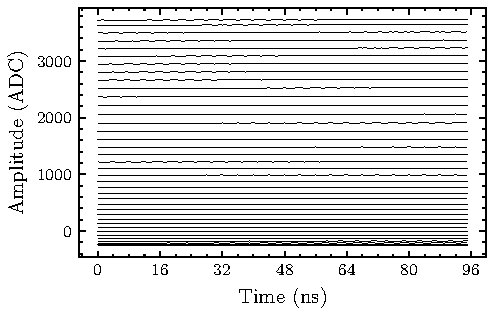
\includegraphics[width=\textwidth]{generation_t5}
    \caption{DC Transfer Function input, measured with TARGET~5.}
    \label{fig:generation_t5}
  \end{subfigure}
  \hfill
  \begin{subfigure}[b]{0.49\textwidth}
    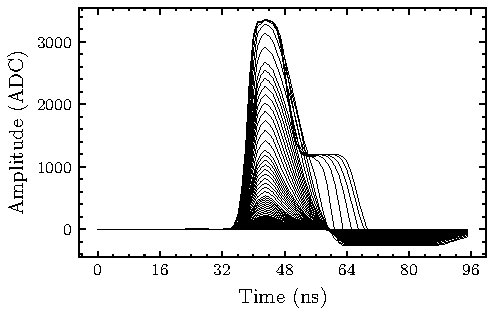
\includegraphics[width=\textwidth]{generation_tc}
    \caption{AC Transfer Function input, measured with TARGET~C.}
    \label{fig:generation_tc}
  \end{subfigure}
  \caption[Transfer Function generation waveforms.]{Multiple average waveforms, increasing in amplitude. Each average contains 1000 waveforms from the same single channel. These waveforms cover the full dynamic range of the TARGET ASIC, and are used as inputs to generate the DC and AC Transfer Functions, respectively.}
\end{figure}

\begin{figure}
  \begin{subfigure}[b]{0.49\textwidth}
    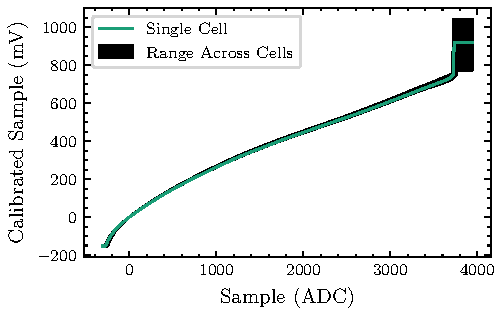
\includegraphics[width=\textwidth]{lookup_t5}
    \caption{DC Transfer Function lookup table, measured with TARGET~5. Contains 64 Transfer Functions, one for each Sampling Cell.}
    \label{fig:lookup_t5}
  \end{subfigure}
  \hfill
  \begin{subfigure}[b]{0.49\textwidth}
    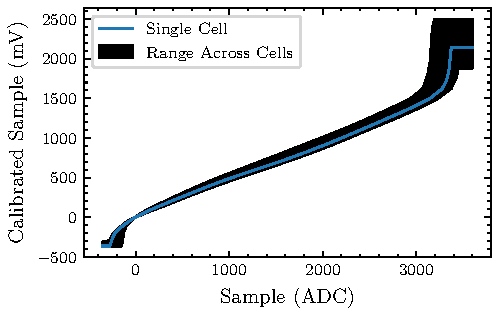
\includegraphics[width=\textwidth]{lookup_tc}
    \caption{AC Transfer Function lookup table, measured with TARGET~C. Contains 4,096 Transfer Functions, one for each Storage Cell.}
    \label{fig:lookup_tc}
  \end{subfigure}
  \caption[Transfer Function lookup tables.]{The Transfer Function lookup tables for a single channel.}
\end{figure}

\subsubsection{Generation (\gls{dc} Transfer Function)}

During the commissioning of \gls{chec-m}, a \gls{dc} Transfer Function was used with no \gls{ac} corrections. To generate this Transfer Function the internal input pedestal voltage (Vped) setting is used to apply a \gls{dc} voltage offset of known amplitude. By repeating the process for Vped values from 500~mV to 1700~mV, in steps of 25~mV, the full dynamic range of the module is explored, covering the range -250~ADC to 3700~ADC (Figure~\ref{generation_t5}). The running averages of the ADC samples are grouped and monitored according to $[Module, Channel, Sampling~Cell, Input~Amplitude]$, utilising every sample in the waveform. Around 1,000 events are required to provide sufficient statistics.

The second step in the generation is to linearly interpolate the running averages at the ADC points defined by the user. This provides a lookup table of mV values with dimensions $[Module, Channel, Sampling~Cell, ADC~Value]$ that can be used to provide a calibrated value for a measured ADC value. The lookup table for a single channel is illustrated in Figure~\change{add figure}. This table is saved to a \gls{fits} file, ready for application.

\subsubsection{Generation (\gls{ac} Transfer Function)}

As the ability to internally set a \gls{dc} voltage with a known amplitude via the Vped was made more difficult in \gls{targetc} (see \ref{ch2-mechanics}) \change{more precise ref, and remember to mention this change}, and the ability to input a \gls{dc} voltage externally is prohibited by the \gls{ac} coupling of the module \change{remember to introduce ac coupling}, the decision was made to transition to an \gls{ac} Transfer Function that uses the expected pulse shape as an input. This approach therefore corrects for the \gls{ac} effect with the appropriate frequency. 
	
The full dynamic range is once again explored, by injecting pulses of a variety of amplitudes. In order to extract the values that correspond to negative amplitudes in this method, the amplitude of the input undershoot is also monitored. Only the samples that corresponds to the maximum of the input pulse (and minimum of the undershoot) has a "true" amplitude of the input amplitude. Therefore to extract the correct samples, each waveform is fitted with two Landau functions, a fair approximation to the pulse shape (Figure~\change{figure showing the fit}). Consequently, only two samples are extracted per waveform, requiring a much larger population of events (\~200,000) in order to generate a reliable running average grouped according to $[Module, Channel, Storage Cell, Input Amplitude]$. It is important to note that a Transfer Function per storage cell was adopted for \gls{targetc}, as it was found to significantly improve the residuals (see \change{appendix tf investigations} for further discussion).

The second step in the generation is identical to the \gls{dc} Transfer Function. The resulting lookup tables can be seen in Figures~\& \change{add figures}.

\subsubsection{Application}

Irrespective of the Transfer Function type, they are stored in a format which enables them to be applied identically. When calibrating an ADC sample, the relevant lookup table is obtained according to the channel and cell of the sample, and is linearly interpolated to provide the calibrated mV value for that ADC value.

\subsubsection{Performance}

Due to its complexity and variety of approaches, the Transfer Function is still one of the most actively discussed aspects of the \gls{chec} calibration, and is most certainly the area where the majority of improvements can be made. Some possibilities for improvement include:
\begin{itemize}
	\item An improved sample extraction method for the \gls{ac} Transfer Function Waveform
	\item Possibilities for a \gls{dc} approach for \gls{targetc}
	\item Returning to the approach described in \cite{Albert2017} where the pedestal is included inside the Transfer Function
	\item Alternatives to linear interpolation, such as Piecewise Cubic Hermite Interpolating Polynomial (PCHIP)
	\item Exchanging the lookup table for a parametrised regression characterisation of the Transfer Function
	\item Decision between "per storage cell" or "per sampling cell"
	\item Inclusion of temperature corrections
\end{itemize}
Appendix~\change{tf investigations} provides some insight into the current progression in these active investigations.

Assessing the performance of the Transfer Functions is a more complicated task than for the pedestals. This is largely because instead of a comparison to a null signal, we are instead comparing to an input amplitude which contains its own uncertainty, and could potentially be incorrect. So while the residuals of the Transfer Function may be small, this does not necessarily mean the calibration is accurate. Therefore the most decisive performance indicator should be one that provides an independent measurement on the ``correct'' amplitude. The most obvious scheme fitting this requirement is the charge resolution, described in \ref{ch3-architecture}. However, while it does hold the drawbacks just mentioned, investigating the residuals through the \gls{rmse} can provide insights on the Transfer Function calibrated unhindered by other components in the detector chain. Figure~\change{insert figure} demonstrates the \gls{rmse} for the presently adopted Transfer Functions for \gls{targetc}, compared to a simple calibration with a fixed conversion value $X~mv/ADC$ \change{obtain sensible value, and talk about the result a bit, non-linearity, show equation for RMSE}.

\notes[inline]{For ch7: Remember to talk about how the MC charge resolution provides us insight into performance with perfect Transfer Functions}

\section{Laboratory Calibration}

\change[inline]{Need lab description in ch2}

\section{Filter-Wheel}

\subsection{Illumination Profile}

\subsection{Camera Geometry}

\section{Photosensor Calibration}

The other primary component in the detector chain that requires calibration is the photosensor itself. As photosensors are a much more common instrument used in a variety of experiments, the calibration procedures typically already exist, and it is a simple case of adapting them to fit our needs.

However, unlike with the \gls{target} modules, where the procedures are very similar between \gls{chec-m} and \gls{chec-s}, an \gls{mapmt} is very different to a \gls{sipmt}. Therefore it is logical to deal with the calibration procedure for each of these photosensors separately.

\subsection{CHEC-M}

Photomultiplier tubes have been widely used in Gamma-ray Astronomy since the first \glspl{iact} \change{get source}, therefore the characterisation of these devices is very well understood. However, \glspl{mapmt} are a more recent evolution of the devices, and although they have the same underlying concept, they do suffer from some limitations, such as the inability to tweak the \gls{hv} on a pixel level, and the electrical crosstalk across the tightly packed pixels \change{check checm paper for other limitations}.

A common method to characterize \glspl{mapmt}, and the one we also adopted, is the use of the \gls{spe} spectrum. The primary result this spectrum provides is the per-pixel value to calibrate from the measured signal in mV (or mV*ns for integrated charge) to \gls{pe}. This conversion value is hereafter referred to as the \gls{spe} value. In order to investigate this parameter, the photosensor is illuminated with a very low light level (average illumination <1~p.e. per pixel). As the photosensor is essentially a photon counting device, the individual peaks of the photoelectrons that are produced by the photocathode can be identified in the histogram of charge amplitudes. The \gls{spe} value is therefore the average charge of the first photoelectron peak. However, the resolution of these peaks can be quite poor, especially for \glspl{mapmt}, therefore the resulting distribution is fit with a function that characterises the photosensor: \change[inline]{add equation for mapm spe fit, and reference its origin}

\change[inline]{SPE fit plots}

This SPE value is proportional to the gain of the photomultiplier, and therefore also proportional to the \gls{hv} applied across the photomultiplier. In order to extract a clear \gls{spe} spectrum, the voltage across the \glspl{mapmt} are set to the maximum value of 1100~V, thereby maximising the separation between the photoelectron and pedestal peaks.

In order to extrapolate the correct \gls{spe} value for other \gls{hv} settings, the following relation:

Can be used in combination with a logarithmic \change{double check, maybe linear regression in log space?} fit of a dataset where the amplitude is measured as a function of HV to obtain $\alpha$ per pixel. \change{include plot of relation}

\change{plots of the SPE values at different hv sets}

In order to apply this calibration, the \gls{spe} value (with units of $mV*ns*p.e.^{-1}$) per pixel is multiplied by the charge extracted per pixel. \change[inline]{show a waveform with this factor applied, maybe also the spectrum}

\subsection{CHEC-S}

In the transition to \glspl{sipmt}, the calibration procedure for the photosensors was revised to better utilise the upgraded functionality of \gls{chec-s}. 

\subsubsection{Gain Matching}

Firstly, the voltages across the photosensors are now configurable per superpixel (group of 4 pixels) \change{mention superpixels in ch3} as opposed to per module. This allows the voltage to be fine-tuned to produce an identical gain response on a per superpixel level.

The procedure for this is illustrated in Figure~\change{gain matching figure}:
\begin{itemize}
	\item The camera is illuminated with approximately 50~p.e.
	\item The waveforms are readout and averaged per superpixel (excluding any dead pixels)
	\item The next voltage settings are calculated such that they will reduce the spread in the pulse height of the averaged waveforms
	\item The new voltage setting are applied, and the process is repeated
\end{itemize}
This iterating approach reduces the gain spread between pixels from \change{values} (Figure~\change{add final comparison figure})

\change[inline]{need a note here or in ch2 about how other parameters of an sipmt change with hv}

The additional benefit of this calibration is that changes in temperature, which would normally affect the gain, can be accounted for by changing the \gls{hv}, therefore maintaining a constant gain response across the camera. This particular in-situ calibration has not yet been implemented, but is intended for the future.

\change[inline]{plot with gain vs temperature?}

\subsubsection{SPE Calibration}

The second step in the \gls{chec-s} photosensor calibration differs according to the purpose of the dataset being calibrated. In order to completely characterise the camera, and produce the Charge Resolution results, the per-pixel \gls{spe} value must be obtained, and used to produce the absolute charge in a waveform (the complete Charge Resolution procedure can be found in Chapter~\ref{ch8-pipeline}).

The function that characterises the \gls{spe} distribution of an \gls{sipmt} is not wildly different to that of an \gls{mapmt}, but does include the significant contribution of the optical crosstalk:
\change[inline]{write function}

The other significant difference in the \gls{spe} distribution of an \gls{sipmt} is the improved resolution of the peaks. Typically when an \gls{sipmt} is illuminated at \change{illumination}, peaks from \change{range of peaks} can be identified. Figure~\change{obtain spe figure of sipm on its own} shows the \gls{spe} spectrum for the model of \gls{sipmt} we have installed into the camera. However, due to the inclusion of the other electronics in the camera, this improved resolution is considerately suppressed, but is still significantly better than observed with \gls{chec-m}\change{reference chec-m figure}.

Figure~\change{insert figure} shows the \gls{spe} spectrum and fit for a pixel in our camera. The resulting parameters are \change[inline]{talk about the spe fit parameters, and show some histograms}

\subsubsection{Flat-Fielding}

Alternatively, in the default data-taking mode of on-sky Cherenkov images, the flat-fielding approach will be used. This exists as a software extension to the gain-matching to further unify the response across the camera. With an illumination of approximately 50 p.e. (as with the gain matching), the coefficients are extracted such that the charge measured in each pixel is the same (after accounting for the difference in illumination between pixels due to the beam profile and curved geometry of the focal plane). These coefficients differ in those obtained via the \gls{spe} method as they include the relative \gls{pde} between pixels in the correction. 

The argument between flat-fielding according to gain response (\gls{spe} fitting) or according to illumination response (method we are adopting) is a common one among \glspl{iact} \change{find references where HESS/MAGIC differ in their approach}, and is also a current topic among the different \gls{cta} telescopes. The reason we have chosen to adopt the latter is it reduces the pixel-to-pixel variations in their response to being illuminated, which is important for Cherenkov shower images. The measured charge in each pixel will not be exactly representative of the number of photoelectrons, but instead it will be representative of the number of photons. However, in order to keep the charge extracted in relatable units, a single nominal $mV*ns*p.e.^{-1}$ conversion value will be applied to the entire camera.

\change[inline]{needs some demonstration of its impact, some plots for example, that continue on from the gain matching plots}

\section{Other}

\change[inline]{remove this section, move subsections higher}
In addition to the calibrations mentioned thus far, there are a few less important calibrations that could improve the performance further. 

\subsection{Timing Corrections}

Due to the routing of the electronics in the front-end, the electrical signal path is slightly different per channel, causing a small difference in apparent arrival of the pulse in the waveform. The relative arrival time per pixel can be seen in Figure~\change{add camera image showing relative time}. 

Not only does this need to be taken into consideration when investigating the timing performance, it also can have a significant impact on the charge extraction, which typically relies on other pixels (neighbouring or entire camera, see Chapter~\ref{ch6-reduction}) sharing an compatible pulse time. The effect of a 1~ns incorrectly extracted charge (when the peak finding is done using the waveforms from all pixels) can have the impact on the charge resolution shown in Figure~\change{show impact of an incorrect time extraction on charge resolution, maybe of just TM?}

The first approach in correcting for this effect is to shift the charge extraction by the timing correction. However, current charge extraction methods do not operate on time scales smaller than the waveform binning, therefore approaches on how to adapt those methods for corrections below that scale are being discussed.

\subsection{\label{temperature_corrections}Temperature Corrections}

Temperature is most likely the most prominent factor in changing the calibration values on short scales, and has been mentioned in almost every approach. Investigations into exactly how these parameters change with temperature are ongoing, but examples can be seen in:
\begin{itemize}
	\item Figure~\change[inline]{Pedestal ramp}
	\item Figure~\change[inline]{TF Variation with temp}
	\item Figure~\change[inline]{Gain variation with temp}
\end{itemize}
In the future we intend to have a calibration pipeline that is independent of these temperature effects. For the photosensors this is very simple, as the voltage across them can be altered to account for the temperature changes. For the \gls{target} modules, this may require an additional lookup table, or an extra dimension to the existing tables.

\subsection{LED Flashers}

Although not technically a part of the waveform processing chain, the LED flashers have an important role in the calibration pipeline, especially for the final operation of the \gls{chec} cameras in \gls{cta}. Their purpose is to allow us to perform in situ calibration, by uniformly illuminating the camera via reflection in the secondary mirror. However to achieve this, we must characterize and calibrate the LEDs such that we accurately know the illumination they are providing. \change[inline]{include some results on the LED calibration, and also mention their temperature dependence.}

\section{Future}

During the long development of \gls{chec}, the calibration procedure has evolved a lot, and multiple iterations have occurred to either:
\begin{itemize}
	\item accommodate the changes required in the upgrades of hardware (such as from \gls{target5} to \gls{targetc})
	\item simplify the calibration to save on resources
	\item or account for additional factors, thereby improving the calibration (such as the \gls{ac} contribution to the Transfer Functions)
\end{itemize}
Therefore, while each iteration improves in one aspect, it may be at the expense of the others. As a result, the \gls{target} calibration procedure described in this chapter appears quite complicated compared to the approaches detailed in \cite{Bechtol2012} and \cite{Albert2017}. The primary next step in the calibration development for \gls{chec} is therefore to review the procedure used, with the aim to produce an approach that is simpler, includes aspects such as temperature dependence, and meets the requirements and processing rates required by \gls{cta}.
